\documentclass[1p]{elsarticle_modified}
%\bibliographystyle{elsarticle-num}

%\usepackage[colorlinks]{hyperref}
%\usepackage{abbrmath_seonhwa} %\Abb, \Ascr, \Acal ,\Abf, \Afrak
\usepackage{amsfonts}
\usepackage{amssymb}
\usepackage{amsmath}
\usepackage{amsthm}
\usepackage{scalefnt}
\usepackage{amsbsy}
\usepackage{kotex}
\usepackage{caption}
\usepackage{subfig}
\usepackage{color}
\usepackage{graphicx}
\usepackage{xcolor} %% white, black, red, green, blue, cyan, magenta, yellow
\usepackage{float}
\usepackage{setspace}
\usepackage{hyperref}

\usepackage{tikz}
\usetikzlibrary{arrows}

\usepackage{multirow}
\usepackage{array} % fixed length table
\usepackage{hhline}

%%%%%%%%%%%%%%%%%%%%%
\makeatletter
\renewcommand*\env@matrix[1][\arraystretch]{%
	\edef\arraystretch{#1}%
	\hskip -\arraycolsep
	\let\@ifnextchar\new@ifnextchar
	\array{*\c@MaxMatrixCols c}}
\makeatother %https://tex.stackexchange.com/questions/14071/how-can-i-increase-the-line-spacing-in-a-matrix
%%%%%%%%%%%%%%%

\usepackage[normalem]{ulem}

\newcommand{\msout}[1]{\ifmmode\text{\sout{\ensuremath{#1}}}\else\sout{#1}\fi}
%SOURCE: \msout is \stkout macro in https://tex.stackexchange.com/questions/20609/strikeout-in-math-mode

\newcommand{\cancel}[1]{
	\ifmmode
	{\color{red}\msout{#1}}
	\else
	{\color{red}\sout{#1}}
	\fi
}

\newcommand{\add}[1]{
	{\color{blue}\uwave{#1}}
}

\newcommand{\replace}[2]{
	\ifmmode
	{\color{red}\msout{#1}}{\color{blue}\uwave{#2}}
	\else
	{\color{red}\sout{#1}}{\color{blue}\uwave{#2}}
	\fi
}

\newcommand{\Sol}{\mathcal{S}} %segment
\newcommand{\D}{D} %diagram
\newcommand{\A}{\mathcal{A}} %arc


%%%%%%%%%%%%%%%%%%%%%%%%%%%%%5 test

\def\sl{\operatorname{\textup{SL}}(2,\Cbb)}
\def\psl{\operatorname{\textup{PSL}}(2,\Cbb)}
\def\quan{\mkern 1mu \triangleright \mkern 1mu}

\theoremstyle{definition}
\newtheorem{thm}{Theorem}[section]
\newtheorem{prop}[thm]{Proposition}
\newtheorem{lem}[thm]{Lemma}
\newtheorem{ques}[thm]{Question}
\newtheorem{cor}[thm]{Corollary}
\newtheorem{defn}[thm]{Definition}
\newtheorem{exam}[thm]{Example}
\newtheorem{rmk}[thm]{Remark}
\newtheorem{alg}[thm]{Algorithm}

\newcommand{\I}{\sqrt{-1}}
\begin{document}

%\begin{frontmatter}
%
%\title{Boundary parabolic representations of knots up to 8 crossings}
%
%%% Group authors per affiliation:
%\author{Yunhi Cho} 
%\address{Department of Mathematics, University of Seoul, Seoul, Korea}
%\ead{yhcho@uos.ac.kr}
%
%
%\author{Seonhwa Kim} %\fnref{s_kim}}
%\address{Center for Geometry and Physics, Institute for Basic Science, Pohang, 37673, Korea}
%\ead{ryeona17@ibs.re.kr}
%
%\author{Hyuk Kim}
%\address{Department of Mathematical Sciences, Seoul National University, Seoul 08826, Korea}
%\ead{hyukkim@snu.ac.kr}
%
%\author{Seokbeom Yoon}
%\address{Department of Mathematical Sciences, Seoul National University, Seoul, 08826,  Korea}
%\ead{sbyoon15@snu.ac.kr}
%
%\begin{abstract}
%We find all boundary parabolic representation of knots up to 8 crossings.
%
%\end{abstract}
%\begin{keyword}
%    \MSC[2010] 57M25 
%\end{keyword}
%
%\end{frontmatter}

%\linenumbers
%\tableofcontents
%
\newcommand\colored[1]{\textcolor{white}{\rule[-0.35ex]{0.8em}{1.4ex}}\kern-0.8em\color{red} #1}%
%\newcommand\colored[1]{\textcolor{white}{ #1}\kern-2.17ex	\textcolor{white}{ #1}\kern-1.81ex	\textcolor{white}{ #1}\kern-2.15ex\color{red}#1	}

{\Large $\underline{12a_{0669}~(K12a_{0669})}$}

\setlength{\tabcolsep}{10pt}
\renewcommand{\arraystretch}{1.6}
\vspace{1cm}\begin{tabular}{m{100pt}>{\centering\arraybackslash}m{274pt}}
\multirow{5}{120pt}{
	\centering
	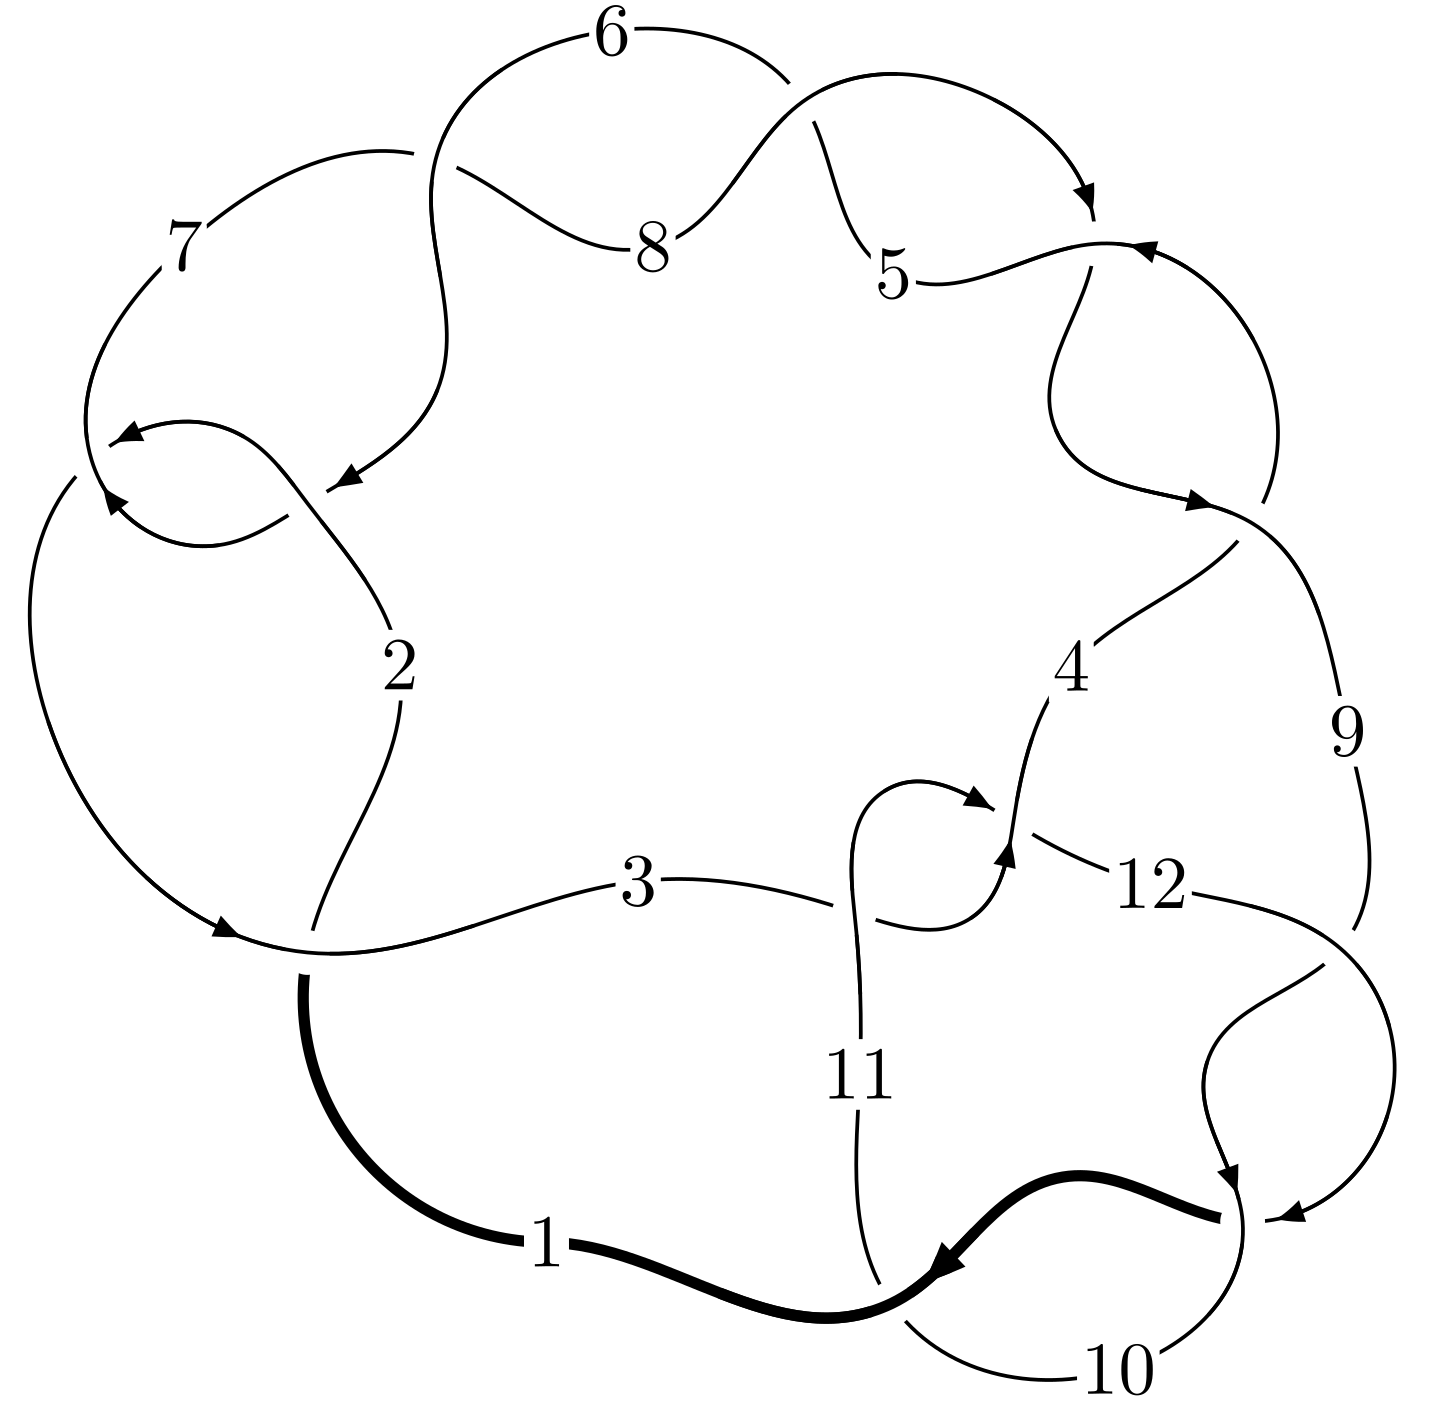
\includegraphics[width=112pt]{../../../GIT/diagram.site/Diagrams/png/1470_12a_0669.png}\\
\ \ \ A knot diagram\footnotemark}&
\allowdisplaybreaks
\textbf{Linearized knot diagam} \\
\cline{2-2}
 &
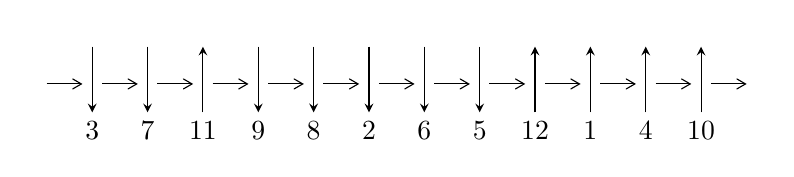
\begin{tikzpicture}[x=20pt, y=17pt]
	% nodes
	\node (C0) at (0, 0) {};
	\node (C1) at (1, 0) {};
	\node (C1U) at (1, +1) {};
	\node (C1D) at (1, -1) {3};

	\node (C2) at (2, 0) {};
	\node (C2U) at (2, +1) {};
	\node (C2D) at (2, -1) {7};

	\node (C3) at (3, 0) {};
	\node (C3U) at (3, +1) {};
	\node (C3D) at (3, -1) {11};

	\node (C4) at (4, 0) {};
	\node (C4U) at (4, +1) {};
	\node (C4D) at (4, -1) {9};

	\node (C5) at (5, 0) {};
	\node (C5U) at (5, +1) {};
	\node (C5D) at (5, -1) {8};

	\node (C6) at (6, 0) {};
	\node (C6U) at (6, +1) {};
	\node (C6D) at (6, -1) {2};

	\node (C7) at (7, 0) {};
	\node (C7U) at (7, +1) {};
	\node (C7D) at (7, -1) {6};

	\node (C8) at (8, 0) {};
	\node (C8U) at (8, +1) {};
	\node (C8D) at (8, -1) {5};

	\node (C9) at (9, 0) {};
	\node (C9U) at (9, +1) {};
	\node (C9D) at (9, -1) {12};

	\node (C10) at (10, 0) {};
	\node (C10U) at (10, +1) {};
	\node (C10D) at (10, -1) {1};

	\node (C11) at (11, 0) {};
	\node (C11U) at (11, +1) {};
	\node (C11D) at (11, -1) {4};

	\node (C12) at (12, 0) {};
	\node (C12U) at (12, +1) {};
	\node (C12D) at (12, -1) {10};
	\node (C13) at (13, 0) {};

	% arrows
	\draw[->,>={angle 60}]
	(C0) edge (C1) (C1) edge (C2) (C2) edge (C3) (C3) edge (C4) (C4) edge (C5) (C5) edge (C6) (C6) edge (C7) (C7) edge (C8) (C8) edge (C9) (C9) edge (C10) (C10) edge (C11) (C11) edge (C12) (C12) edge (C13) ;	\draw[->,>=stealth]
	(C1U) edge (C1D) (C2U) edge (C2D) (C3D) edge (C3U) (C4U) edge (C4D) (C5U) edge (C5D) (C6U) edge (C6D) (C7U) edge (C7D) (C8U) edge (C8D) (C9D) edge (C9U) (C10D) edge (C10U) (C11D) edge (C11U) (C12D) edge (C12U) ;
	\end{tikzpicture} \\
\hhline{~~} \\& 
\textbf{Solving Sequence} \\ \cline{2-2} 
 &
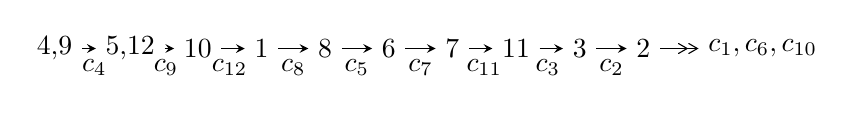
\begin{tikzpicture}[x=23pt, y=7pt]
	% node
	\node (A0) at (-1/8, 0) {4,9};
	\node (A1) at (17/16, 0) {5,12};
	\node (A2) at (17/8, 0) {10};
	\node (A3) at (25/8, 0) {1};
	\node (A4) at (33/8, 0) {8};
	\node (A5) at (41/8, 0) {6};
	\node (A6) at (49/8, 0) {7};
	\node (A7) at (57/8, 0) {11};
	\node (A8) at (65/8, 0) {3};
	\node (A9) at (73/8, 0) {2};
	\node (C1) at (1/2, -1) {$c_{4}$};
	\node (C2) at (13/8, -1) {$c_{9}$};
	\node (C3) at (21/8, -1) {$c_{12}$};
	\node (C4) at (29/8, -1) {$c_{8}$};
	\node (C5) at (37/8, -1) {$c_{5}$};
	\node (C6) at (45/8, -1) {$c_{7}$};
	\node (C7) at (53/8, -1) {$c_{11}$};
	\node (C8) at (61/8, -1) {$c_{3}$};
	\node (C9) at (69/8, -1) {$c_{2}$};
	\node (A10) at (11, 0) {$c_{1},c_{6},c_{10}$};

	% edge
	\draw[->,>=stealth]	
	(A0) edge (A1) (A1) edge (A2) (A2) edge (A3) (A3) edge (A4) (A4) edge (A5) (A5) edge (A6) (A6) edge (A7) (A7) edge (A8) (A8) edge (A9) ;
	\draw[->>,>={angle 60}]	
	(A9) edge (A10);
\end{tikzpicture} \\ 

\end{tabular} \\

\footnotetext{
The image of knot diagram is generated by the software ``\textbf{Draw programme}" developed by Andrew Bartholomew(\url{http://www.layer8.co.uk/maths/draw/index.htm\#Running-draw}), where we modified some parts for our purpose(\url{https://github.com/CATsTAILs/LinksPainter}).
}\phantom \\ \newline 
\centering \textbf{Ideals for irreducible components\footnotemark of $X_{\text{par}}$} 
 
\begin{align*}
I^u_{1}&=\langle 
-25220615118 u^{37}-125516232099 u^{36}+\cdots+42034358527 b-24647116036,\\
\phantom{I^u_{1}}&\phantom{= \langle  }60529476279 u^{37}+353049488728 u^{36}+\cdots+42034358527 a+595728741584,\\
\phantom{I^u_{1}}&\phantom{= \langle  }u^{38}+6 u^{37}+\cdots+16 u+1\rangle \\
I^u_{2}&=\langle 
b,\;- u^4+u^3-4 u^2+a+3 u-3,\;u^5- u^4+4 u^3-3 u^2+3 u-1\rangle \\
\\
\end{align*}
\raggedright * 2 irreducible components of $\dim_{\mathbb{C}}=0$, with total 43 representations.\\
\footnotetext{All coefficients of polynomials are rational numbers. But the coefficients are sometimes approximated in decimal forms when there is not enough margin.}
\newpage
\renewcommand{\arraystretch}{1}
\centering \section*{I. $I^u_{1}= \langle -2.52\times10^{10} u^{37}-1.26\times10^{11} u^{36}+\cdots+4.20\times10^{10} b-2.46\times10^{10},\;6.05\times10^{10} u^{37}+3.53\times10^{11} u^{36}+\cdots+4.20\times10^{10} a+5.96\times10^{11},\;u^{38}+6 u^{37}+\cdots+16 u+1 \rangle$}
\flushleft \textbf{(i) Arc colorings}\\
\begin{tabular}{m{7pt} m{180pt} m{7pt} m{180pt} }
\flushright $a_{4}=$&$\begin{pmatrix}1\\0\end{pmatrix}$ \\
\flushright $a_{9}=$&$\begin{pmatrix}0\\u\end{pmatrix}$ \\
\flushright $a_{5}=$&$\begin{pmatrix}1\\u^2\end{pmatrix}$ \\
\flushright $a_{12}=$&$\begin{pmatrix}-1.44000 u^{37}-8.39907 u^{36}+\cdots-114.524 u-14.1724\\0.600000 u^{37}+2.98604 u^{36}+\cdots+1.86170 u+0.586356\end{pmatrix}$ \\
\flushright $a_{10}=$&$\begin{pmatrix}-1.24000 u^{37}-7.40372 u^{36}+\cdots-102.904 u-12.3103\\0.400000 u^{37}+2.01396 u^{36}+\cdots+2.13830 u+0.413644\end{pmatrix}$ \\
\flushright $a_{1}=$&$\begin{pmatrix}-0.600000 u^{37}-3.00931 u^{36}+\cdots-19.7589 u-3.27576\\0.400000 u^{37}+2.01396 u^{36}+\cdots+2.13830 u+0.413644\end{pmatrix}$ \\
\flushright $a_{8}=$&$\begin{pmatrix}u\\u^3+u\end{pmatrix}$ \\
\flushright $a_{6}=$&$\begin{pmatrix}u^2+1\\u^4+2 u^2\end{pmatrix}$ \\
\flushright $a_{7}=$&$\begin{pmatrix}u^3+2 u\\u^5+3 u^3+u\end{pmatrix}$ \\
\flushright $a_{11}=$&$\begin{pmatrix}-2.04000 u^{37}-11.3851 u^{36}+\cdots-116.386 u-14.7588\\0.600000 u^{37}+2.98604 u^{36}+\cdots+1.86170 u+0.586356\end{pmatrix}$ \\
\flushright $a_{3}=$&$\begin{pmatrix}-1.00434 u^{37}-5.62602 u^{36}+\cdots-39.9468 u-5.08000\\0.590693 u^{37}+3.54416 u^{36}+\cdots+6.32424 u+0.600000\end{pmatrix}$ \\
\flushright $a_{2}=$&$\begin{pmatrix}-1.00000 u^{37}-5.60444 u^{36}+\cdots-30.7482 u-4.28010\\0.400000 u^{37}+2.59513 u^{36}+\cdots+10.9894 u+1.00434\end{pmatrix}$\\&\end{tabular}
\flushleft \textbf{(ii) Obstruction class $= -1$}\\~\\
\flushleft \textbf{(iii) Cusp Shapes $= \frac{323207095835}{42034358527} u^{37}+\frac{1803051253389}{42034358527} u^{36}+\cdots+\frac{12006740049581}{42034358527} u+\frac{1316852383934}{42034358527}$}\\~\\
\newpage\renewcommand{\arraystretch}{1}
\flushleft \textbf{(iv) u-Polynomials at the component}\newline \\
\begin{tabular}{m{50pt}|m{274pt}}
Crossings & \hspace{64pt}u-Polynomials at each crossing \\
\hline $$\begin{aligned}c_{1},c_{4},c_{5}\\c_{7},c_{8}\end{aligned}$$&$\begin{aligned}
&u^{38}+6 u^{37}+\cdots+16 u+1
\end{aligned}$\\
\hline $$\begin{aligned}c_{2},c_{6}\end{aligned}$$&$\begin{aligned}
&u^{38}-2 u^{37}+\cdots+4 u-1
\end{aligned}$\\
\hline $$\begin{aligned}c_{3},c_{11}\end{aligned}$$&$\begin{aligned}
&u^{38}- u^{37}+\cdots-32 u+32
\end{aligned}$\\
\hline $$\begin{aligned}c_{9},c_{10},c_{12}\end{aligned}$$&$\begin{aligned}
&u^{38}+6 u^{37}+\cdots-2 u-1
\end{aligned}$\\
\hline
\end{tabular}\\~\\
\newpage\renewcommand{\arraystretch}{1}
\flushleft \textbf{(v) Riley Polynomials at the component}\newline \\
\begin{tabular}{m{50pt}|m{274pt}}
Crossings & \hspace{64pt}Riley Polynomials at each crossing \\
\hline $$\begin{aligned}c_{1},c_{4},c_{5}\\c_{7},c_{8}\end{aligned}$$&$\begin{aligned}
&y^{38}+54 y^{37}+\cdots-12 y+1
\end{aligned}$\\
\hline $$\begin{aligned}c_{2},c_{6}\end{aligned}$$&$\begin{aligned}
&y^{38}-6 y^{37}+\cdots-16 y+1
\end{aligned}$\\
\hline $$\begin{aligned}c_{3},c_{11}\end{aligned}$$&$\begin{aligned}
&y^{38}-33 y^{37}+\cdots-3584 y+1024
\end{aligned}$\\
\hline $$\begin{aligned}c_{9},c_{10},c_{12}\end{aligned}$$&$\begin{aligned}
&y^{38}-42 y^{37}+\cdots+6 y+1
\end{aligned}$\\
\hline
\end{tabular}\\~\\
\newpage\flushleft \textbf{(vi) Complex Volumes and Cusp Shapes}
$$\begin{array}{c|c|c}  
\text{Solutions to }I^u_{1}& \I (\text{vol} + \sqrt{-1}CS) & \text{Cusp shape}\\
 \hline 
\begin{aligned}
u &= -0.713718 + 0.696674 I \\
a &= \phantom{-}0.98664 + 1.13350 I \\
b &= \phantom{-}1.355910 + 0.254773 I\end{aligned}
 & \phantom{-}6.26346 + 5.04642 I & \phantom{-0.000000 } 0. - 6.40435 I \\ \hline\begin{aligned}
u &= -0.713718 - 0.696674 I \\
a &= \phantom{-}0.98664 - 1.13350 I \\
b &= \phantom{-}1.355910 - 0.254773 I\end{aligned}
 & \phantom{-}6.26346 - 5.04642 I & \phantom{-0.000000 -}0. + 6.40435 I \\ \hline\begin{aligned}
u &= -0.205081 + 0.964197 I \\
a &= -0.002810 + 0.336869 I \\
b &= -0.045418 + 0.545182 I\end{aligned}
 & \phantom{-}2.26768 + 2.34844 I & \phantom{-0.000000 } 0. - 4.01424 I \\ \hline\begin{aligned}
u &= -0.205081 - 0.964197 I \\
a &= -0.002810 - 0.336869 I \\
b &= -0.045418 - 0.545182 I\end{aligned}
 & \phantom{-}2.26768 - 2.34844 I & \phantom{-0.000000 -}0. + 4.01424 I \\ \hline\begin{aligned}
u &= -0.861163\phantom{ +0.000000I} \\
a &= \phantom{-}1.70659\phantom{ +0.000000I} \\
b &= \phantom{-}1.30561\phantom{ +0.000000I}\end{aligned}
 & \phantom{-}4.20147\phantom{ +0.000000I} & -0.424720\phantom{ +0.000000I} \\ \hline\begin{aligned}
u &= -0.032507 + 1.171160 I \\
a &= -0.645677 - 0.518349 I \\
b &= \phantom{-}1.192870 - 0.112572 I\end{aligned}
 & \phantom{-}6.07449 + 0.14915 I & \phantom{-0.000000 } 0 \\ \hline\begin{aligned}
u &= -0.032507 - 1.171160 I \\
a &= -0.645677 + 0.518349 I \\
b &= \phantom{-}1.192870 + 0.112572 I\end{aligned}
 & \phantom{-}6.07449 - 0.14915 I & \phantom{-0.000000 } 0 \\ \hline\begin{aligned}
u &= \phantom{-}0.190395 + 1.187080 I \\
a &= -0.038520 + 1.334050 I \\
b &= -1.55601 + 0.43836 I\end{aligned}
 & \phantom{-}13.51030 - 3.29880 I & \phantom{-0.000000 } 0 \\ \hline\begin{aligned}
u &= \phantom{-}0.190395 - 1.187080 I \\
a &= -0.038520 - 1.334050 I \\
b &= -1.55601 - 0.43836 I\end{aligned}
 & \phantom{-}13.51030 + 3.29880 I & \phantom{-0.000000 } 0 \\ \hline\begin{aligned}
u &= -0.119477 + 1.235160 I \\
a &= -0.083865 - 1.148000 I \\
b &= \phantom{-}0.070500 - 1.218200 I\end{aligned}
 & \phantom{-}8.02065 + 2.76566 I & \phantom{-0.000000 } 0\\
 \hline 
 \end{array}$$\newpage$$\begin{array}{c|c|c}  
\text{Solutions to }I^u_{1}& \I (\text{vol} + \sqrt{-1}CS) & \text{Cusp shape}\\
 \hline 
\begin{aligned}
u &= -0.119477 - 1.235160 I \\
a &= -0.083865 + 1.148000 I \\
b &= \phantom{-}0.070500 + 1.218200 I\end{aligned}
 & \phantom{-}8.02065 - 2.76566 I & \phantom{-0.000000 } 0 \\ \hline\begin{aligned}
u &= -0.223356 + 1.231840 I \\
a &= \phantom{-}0.531548 - 0.533329 I \\
b &= -1.185810 - 0.238140 I\end{aligned}
 & \phantom{-}5.79827 + 5.29458 I & \phantom{-0.000000 } 0 \\ \hline\begin{aligned}
u &= -0.223356 - 1.231840 I \\
a &= \phantom{-}0.531548 + 0.533329 I \\
b &= -1.185810 + 0.238140 I\end{aligned}
 & \phantom{-}5.79827 - 5.29458 I & \phantom{-0.000000 } 0 \\ \hline\begin{aligned}
u &= -0.454460 + 0.526349 I \\
a &= \phantom{-}0.225842 - 0.858062 I \\
b &= -0.810125 - 0.280595 I\end{aligned}
 & \phantom{-}0.14659 + 2.93637 I & -1.27878 - 9.48259 I \\ \hline\begin{aligned}
u &= -0.454460 - 0.526349 I \\
a &= \phantom{-}0.225842 + 0.858062 I \\
b &= -0.810125 + 0.280595 I\end{aligned}
 & \phantom{-}0.14659 - 2.93637 I & -1.27878 + 9.48259 I \\ \hline\begin{aligned}
u &= -0.383220 + 1.338060 I \\
a &= \phantom{-}0.143279 + 1.122790 I \\
b &= \phantom{-}1.48427 + 0.49972 I\end{aligned}
 & \phantom{-}12.7262 + 8.9717 I & \phantom{-0.000000 } 0 \\ \hline\begin{aligned}
u &= -0.383220 - 1.338060 I \\
a &= \phantom{-}0.143279 - 1.122790 I \\
b &= \phantom{-}1.48427 - 0.49972 I\end{aligned}
 & \phantom{-}12.7262 - 8.9717 I & \phantom{-0.000000 } 0 \\ \hline\begin{aligned}
u &= -0.242924 + 0.500540 I \\
a &= -0.77914 - 2.00057 I \\
b &= \phantom{-}0.217646 - 0.715322 I\end{aligned}
 & \phantom{-}2.34679 + 1.50207 I & \phantom{-}1.29303 - 3.53914 I \\ \hline\begin{aligned}
u &= -0.242924 - 0.500540 I \\
a &= -0.77914 + 2.00057 I \\
b &= \phantom{-}0.217646 + 0.715322 I\end{aligned}
 & \phantom{-}2.34679 - 1.50207 I & \phantom{-}1.29303 + 3.53914 I \\ \hline\begin{aligned}
u &= \phantom{-}0.390857 + 0.382528 I \\
a &= -1.94196 + 2.07024 I \\
b &= -1.47608 + 0.13954 I\end{aligned}
 & \phantom{-}8.43405 - 1.32281 I & \phantom{-}8.28038 + 0.36190 I\\
 \hline 
 \end{array}$$\newpage$$\begin{array}{c|c|c}  
\text{Solutions to }I^u_{1}& \I (\text{vol} + \sqrt{-1}CS) & \text{Cusp shape}\\
 \hline 
\begin{aligned}
u &= \phantom{-}0.390857 - 0.382528 I \\
a &= -1.94196 - 2.07024 I \\
b &= -1.47608 - 0.13954 I\end{aligned}
 & \phantom{-}8.43405 + 1.32281 I & \phantom{-}8.28038 - 0.36190 I \\ \hline\begin{aligned}
u &= -0.468337 + 0.127698 I \\
a &= -0.182428 + 0.431853 I \\
b &= -0.370032 + 0.319434 I\end{aligned}
 & -1.073810 + 0.172026 I & -9.19796 - 0.41861 I \\ \hline\begin{aligned}
u &= -0.468337 - 0.127698 I \\
a &= -0.182428 - 0.431853 I \\
b &= -0.370032 - 0.319434 I\end{aligned}
 & -1.073810 - 0.172026 I & -9.19796 + 0.41861 I \\ \hline\begin{aligned}
u &= -0.05162 + 1.71260 I \\
a &= \phantom{-}0.001886 + 0.320518 I \\
b &= -0.001031 + 0.619536 I\end{aligned}
 & \phantom{-}11.82160 + 3.35648 I & \phantom{-0.000000 } 0 \\ \hline\begin{aligned}
u &= -0.05162 - 1.71260 I \\
a &= \phantom{-}0.001886 - 0.320518 I \\
b &= -0.001031 - 0.619536 I\end{aligned}
 & \phantom{-}11.82160 - 3.35648 I & \phantom{-0.000000 } 0 \\ \hline\begin{aligned}
u &= -0.031423 + 0.280285 I \\
a &= -1.24282 - 2.10298 I \\
b &= \phantom{-}0.728609 + 0.020401 I\end{aligned}
 & \phantom{-}1.222660 - 0.148523 I & \phantom{-}6.95502 - 0.36222 I \\ \hline\begin{aligned}
u &= -0.031423 - 0.280285 I \\
a &= -1.24282 + 2.10298 I \\
b &= \phantom{-}0.728609 - 0.020401 I\end{aligned}
 & \phantom{-}1.222660 + 0.148523 I & \phantom{-}6.95502 + 0.36222 I \\ \hline\begin{aligned}
u &= -0.00837 + 1.78126 I \\
a &= -0.528064 - 0.356522 I \\
b &= \phantom{-}1.45222 - 0.21060 I\end{aligned}
 & \phantom{-}16.9093 + 0.3307 I & \phantom{-0.000000 } 0 \\ \hline\begin{aligned}
u &= -0.00837 - 1.78126 I \\
a &= -0.528064 + 0.356522 I \\
b &= \phantom{-}1.45222 + 0.21060 I\end{aligned}
 & \phantom{-}16.9093 - 0.3307 I & \phantom{-0.000000 } 0 \\ \hline\begin{aligned}
u &= \phantom{-}0.04878 + 1.78515 I \\
a &= \phantom{-}0.151260 + 0.916668 I \\
b &= -1.62783 + 0.66338 I\end{aligned}
 & -15.0990 - 4.3588 I & \phantom{-0.000000 } 0\\
 \hline 
 \end{array}$$\newpage$$\begin{array}{c|c|c}  
\text{Solutions to }I^u_{1}& \I (\text{vol} + \sqrt{-1}CS) & \text{Cusp shape}\\
 \hline 
\begin{aligned}
u &= \phantom{-}0.04878 - 1.78515 I \\
a &= \phantom{-}0.151260 - 0.916668 I \\
b &= -1.62783 - 0.66338 I\end{aligned}
 & -15.0990 + 4.3588 I & \phantom{-0.000000 } 0 \\ \hline\begin{aligned}
u &= -0.05643 + 1.79298 I \\
a &= \phantom{-}0.514785 - 0.362719 I \\
b &= -1.44825 - 0.23847 I\end{aligned}
 & \phantom{-}16.8561 + 6.5503 I & \phantom{-0.000000 } 0 \\ \hline\begin{aligned}
u &= -0.05643 - 1.79298 I \\
a &= \phantom{-}0.514785 + 0.362719 I \\
b &= -1.44825 + 0.23847 I\end{aligned}
 & \phantom{-}16.8561 - 6.5503 I & \phantom{-0.000000 } 0 \\ \hline\begin{aligned}
u &= -0.03067 + 1.79505 I \\
a &= -0.010921 - 0.875007 I \\
b &= \phantom{-}0.01525 - 1.51868 I\end{aligned}
 & \phantom{-}19.1652 + 3.4491 I & \phantom{-0.000000 } 0 \\ \hline\begin{aligned}
u &= -0.03067 - 1.79505 I \\
a &= -0.010921 + 0.875007 I \\
b &= \phantom{-}0.01525 + 1.51868 I\end{aligned}
 & \phantom{-}19.1652 - 3.4491 I & \phantom{-0.000000 } 0 \\ \hline\begin{aligned}
u &= -0.10251 + 1.82008 I \\
a &= -0.126790 + 0.897308 I \\
b &= \phantom{-}1.60864 + 0.67923 I\end{aligned}
 & -15.2648 + 11.2768 I & \phantom{-0.000000 } 0 \\ \hline\begin{aligned}
u &= -0.10251 - 1.82008 I \\
a &= -0.126790 - 0.897308 I \\
b &= \phantom{-}1.60864 - 0.67923 I\end{aligned}
 & -15.2648 - 11.2768 I & \phantom{-0.000000 } 0 \\ \hline\begin{aligned}
u &= -0.150697\phantom{ +0.000000I} \\
a &= -5.65109\phantom{ +0.000000I} \\
b &= \phantom{-}0.483736\phantom{ +0.000000I}\end{aligned}
 & \phantom{-}1.16378\phantom{ +0.000000I} & \phantom{-}11.6280\phantom{ +0.000000I}\\
 \hline 
 \end{array}$$\newpage\newpage\renewcommand{\arraystretch}{1}
\centering \section*{II. $I^u_{2}= \langle b,\;- u^4+u^3-4 u^2+a+3 u-3,\;u^5- u^4+4 u^3-3 u^2+3 u-1 \rangle$}
\flushleft \textbf{(i) Arc colorings}\\
\begin{tabular}{m{7pt} m{180pt} m{7pt} m{180pt} }
\flushright $a_{4}=$&$\begin{pmatrix}1\\0\end{pmatrix}$ \\
\flushright $a_{9}=$&$\begin{pmatrix}0\\u\end{pmatrix}$ \\
\flushright $a_{5}=$&$\begin{pmatrix}1\\u^2\end{pmatrix}$ \\
\flushright $a_{12}=$&$\begin{pmatrix}u^4- u^3+4 u^2-3 u+3\\0\end{pmatrix}$ \\
\flushright $a_{10}=$&$\begin{pmatrix}u^4- u^3+4 u^2-3 u+3\\u\end{pmatrix}$ \\
\flushright $a_{1}=$&$\begin{pmatrix}0\\- u\end{pmatrix}$ \\
\flushright $a_{8}=$&$\begin{pmatrix}u\\u^3+u\end{pmatrix}$ \\
\flushright $a_{6}=$&$\begin{pmatrix}u^2+1\\u^4+2 u^2\end{pmatrix}$ \\
\flushright $a_{7}=$&$\begin{pmatrix}u^3+2 u\\u^4- u^3+3 u^2-2 u+1\end{pmatrix}$ \\
\flushright $a_{11}=$&$\begin{pmatrix}u^4- u^3+4 u^2-3 u+3\\0\end{pmatrix}$ \\
\flushright $a_{3}=$&$\begin{pmatrix}1\\0\end{pmatrix}$ \\
\flushright $a_{2}=$&$\begin{pmatrix}u\\- u\end{pmatrix}$\\&\end{tabular}
\flushleft \textbf{(ii) Obstruction class $= 1$}\\~\\
\flushleft \textbf{(iii) Cusp Shapes $= -7 u^4+6 u^3-28 u^2+17 u-12$}\\~\\
\newpage\renewcommand{\arraystretch}{1}
\flushleft \textbf{(iv) u-Polynomials at the component}\newline \\
\begin{tabular}{m{50pt}|m{274pt}}
Crossings & \hspace{64pt}u-Polynomials at each crossing \\
\hline $$\begin{aligned}c_{1},c_{4},c_{5}\end{aligned}$$&$\begin{aligned}
&u^5- u^4+4 u^3-3 u^2+3 u-1
\end{aligned}$\\
\hline $$\begin{aligned}c_{2}\end{aligned}$$&$\begin{aligned}
&u^5- u^4+u^2+u-1
\end{aligned}$\\
\hline $$\begin{aligned}c_{3},c_{11}\end{aligned}$$&$\begin{aligned}
&u^5
\end{aligned}$\\
\hline $$\begin{aligned}c_{6}\end{aligned}$$&$\begin{aligned}
&u^5+u^4- u^2+u+1
\end{aligned}$\\
\hline $$\begin{aligned}c_{7},c_{8}\end{aligned}$$&$\begin{aligned}
&u^5+u^4+4 u^3+3 u^2+3 u+1
\end{aligned}$\\
\hline $$\begin{aligned}c_{9},c_{10}\end{aligned}$$&$\begin{aligned}
&(u+1)^5
\end{aligned}$\\
\hline $$\begin{aligned}c_{12}\end{aligned}$$&$\begin{aligned}
&(u-1)^5
\end{aligned}$\\
\hline
\end{tabular}\\~\\
\newpage\renewcommand{\arraystretch}{1}
\flushleft \textbf{(v) Riley Polynomials at the component}\newline \\
\begin{tabular}{m{50pt}|m{274pt}}
Crossings & \hspace{64pt}Riley Polynomials at each crossing \\
\hline $$\begin{aligned}c_{1},c_{4},c_{5}\\c_{7},c_{8}\end{aligned}$$&$\begin{aligned}
&y^5+7 y^4+16 y^3+13 y^2+3 y-1
\end{aligned}$\\
\hline $$\begin{aligned}c_{2},c_{6}\end{aligned}$$&$\begin{aligned}
&y^5- y^4+4 y^3-3 y^2+3 y-1
\end{aligned}$\\
\hline $$\begin{aligned}c_{3},c_{11}\end{aligned}$$&$\begin{aligned}
&y^5
\end{aligned}$\\
\hline $$\begin{aligned}c_{9},c_{10},c_{12}\end{aligned}$$&$\begin{aligned}
&(y-1)^5
\end{aligned}$\\
\hline
\end{tabular}\\~\\
\newpage\flushleft \textbf{(vi) Complex Volumes and Cusp Shapes}
$$\begin{array}{c|c|c}  
\text{Solutions to }I^u_{2}& \I (\text{vol} + \sqrt{-1}CS) & \text{Cusp shape}\\
 \hline 
\begin{aligned}
u &= \phantom{-}0.233677 + 0.885557 I \\
a &= \phantom{-}0.278580 - 1.055720 I \\
b &= \phantom{-0.000000 } 0\end{aligned}
 & \phantom{-}3.46474 - 2.21397 I & \phantom{-}6.65223 + 4.39723 I \\ \hline\begin{aligned}
u &= \phantom{-}0.233677 - 0.885557 I \\
a &= \phantom{-}0.278580 + 1.055720 I \\
b &= \phantom{-0.000000 } 0\end{aligned}
 & \phantom{-}3.46474 + 2.21397 I & \phantom{-}6.65223 - 4.39723 I \\ \hline\begin{aligned}
u &= \phantom{-}0.416284\phantom{ +0.000000I} \\
a &= \phantom{-}2.40221\phantom{ +0.000000I} \\
b &= \phantom{-0.000000 } 0\end{aligned}
 & \phantom{-}0.762751\phantom{ +0.000000I} & -9.55270\phantom{ +0.000000I} \\ \hline\begin{aligned}
u &= \phantom{-}0.05818 + 1.69128 I \\
a &= \phantom{-}0.020316 - 0.590570 I \\
b &= \phantom{-0.000000 } 0\end{aligned}
 & \phantom{-}12.60320 - 3.33174 I & \phantom{-}9.12414 + 2.18947 I \\ \hline\begin{aligned}
u &= \phantom{-}0.05818 - 1.69128 I \\
a &= \phantom{-}0.020316 + 0.590570 I \\
b &= \phantom{-0.000000 } 0\end{aligned}
 & \phantom{-}12.60320 + 3.33174 I & \phantom{-}9.12414 - 2.18947 I\\
 \hline 
 \end{array}$$\newpage
\newpage\renewcommand{\arraystretch}{1}
\centering \section*{ III. u-Polynomials}
\begin{tabular}{m{50pt}|m{274pt}}
Crossings & \hspace{64pt}u-Polynomials at each crossing \\
\hline $$\begin{aligned}c_{1},c_{4},c_{5}\end{aligned}$$&$\begin{aligned}
&(u^5- u^4+4 u^3-3 u^2+3 u-1)(u^{38}+6 u^{37}+\cdots+16 u+1)
\end{aligned}$\\
\hline $$\begin{aligned}c_{2}\end{aligned}$$&$\begin{aligned}
&(u^5- u^4+u^2+u-1)(u^{38}-2 u^{37}+\cdots+4 u-1)
\end{aligned}$\\
\hline $$\begin{aligned}c_{3},c_{11}\end{aligned}$$&$\begin{aligned}
&u^5(u^{38}- u^{37}+\cdots-32 u+32)
\end{aligned}$\\
\hline $$\begin{aligned}c_{6}\end{aligned}$$&$\begin{aligned}
&(u^5+u^4- u^2+u+1)(u^{38}-2 u^{37}+\cdots+4 u-1)
\end{aligned}$\\
\hline $$\begin{aligned}c_{7},c_{8}\end{aligned}$$&$\begin{aligned}
&(u^5+u^4+4 u^3+3 u^2+3 u+1)(u^{38}+6 u^{37}+\cdots+16 u+1)
\end{aligned}$\\
\hline $$\begin{aligned}c_{9},c_{10}\end{aligned}$$&$\begin{aligned}
&((u+1)^5)(u^{38}+6 u^{37}+\cdots-2 u-1)
\end{aligned}$\\
\hline $$\begin{aligned}c_{12}\end{aligned}$$&$\begin{aligned}
&((u-1)^5)(u^{38}+6 u^{37}+\cdots-2 u-1)
\end{aligned}$\\
\hline
\end{tabular}\newpage\renewcommand{\arraystretch}{1}
\centering \section*{ IV. Riley Polynomials}
\begin{tabular}{m{50pt}|m{274pt}}
Crossings & \hspace{64pt}Riley Polynomials at each crossing \\
\hline $$\begin{aligned}c_{1},c_{4},c_{5}\\c_{7},c_{8}\end{aligned}$$&$\begin{aligned}
&(y^5+7 y^4+16 y^3+13 y^2+3 y-1)(y^{38}+54 y^{37}+\cdots-12 y+1)
\end{aligned}$\\
\hline $$\begin{aligned}c_{2},c_{6}\end{aligned}$$&$\begin{aligned}
&(y^5- y^4+4 y^3-3 y^2+3 y-1)(y^{38}-6 y^{37}+\cdots-16 y+1)
\end{aligned}$\\
\hline $$\begin{aligned}c_{3},c_{11}\end{aligned}$$&$\begin{aligned}
&y^5(y^{38}-33 y^{37}+\cdots-3584 y+1024)
\end{aligned}$\\
\hline $$\begin{aligned}c_{9},c_{10},c_{12}\end{aligned}$$&$\begin{aligned}
&((y-1)^5)(y^{38}-42 y^{37}+\cdots+6 y+1)
\end{aligned}$\\
\hline
\end{tabular}
\vskip 2pc
\end{document}